\subsubsection{Iteration 2: Exploration of RL-Based Control (Preliminary)}

This iteration explored the use of a reinforcement learning (RL) agent for hovering control. The goal was to reduce the high-frequency control signals observed in the PID-based approach and provide smoother guidance that better matches human perception.

\paragraph{Design}

A simplified 1D hovering task was implemented, where the agent controlled the vertical position ($y$) to stay within a target band $[H - R, H + R]$. The agent received two observations: a normalized height error and the vertical velocity. A reward function combining event-based and continuous feedback was used to encourage stable hovering behavior.

The agent was trained using Proximal Policy Optimization (PPO) for $5 \times 10^5$ steps. Training progress was monitored through cumulative reward and episode length.

\paragraph{Enactment}

The machine learning process was implemented using Unity's ML-Agents toolkit, which leverages PyTorch as its underlying deep learning framework and provides training analytics for performance evaluation. The results indicate that the agent successfully learned to maintain stable hovering within the designated target range. As shown in Figure~\ref{fig:rl_result}, the cumulative reward increased steadily after approximately 100,000 training steps and plateaued around 400,000 steps. Furthermore, episode length progressively increased over time, suggesting improved flight stability and control performance.

\begin{figure}[H]
    \caption{Training performance of the reinforcement learning agent using PyTorch via Unity ML-Agents.}\label{fig:rl_result}
    \centering
    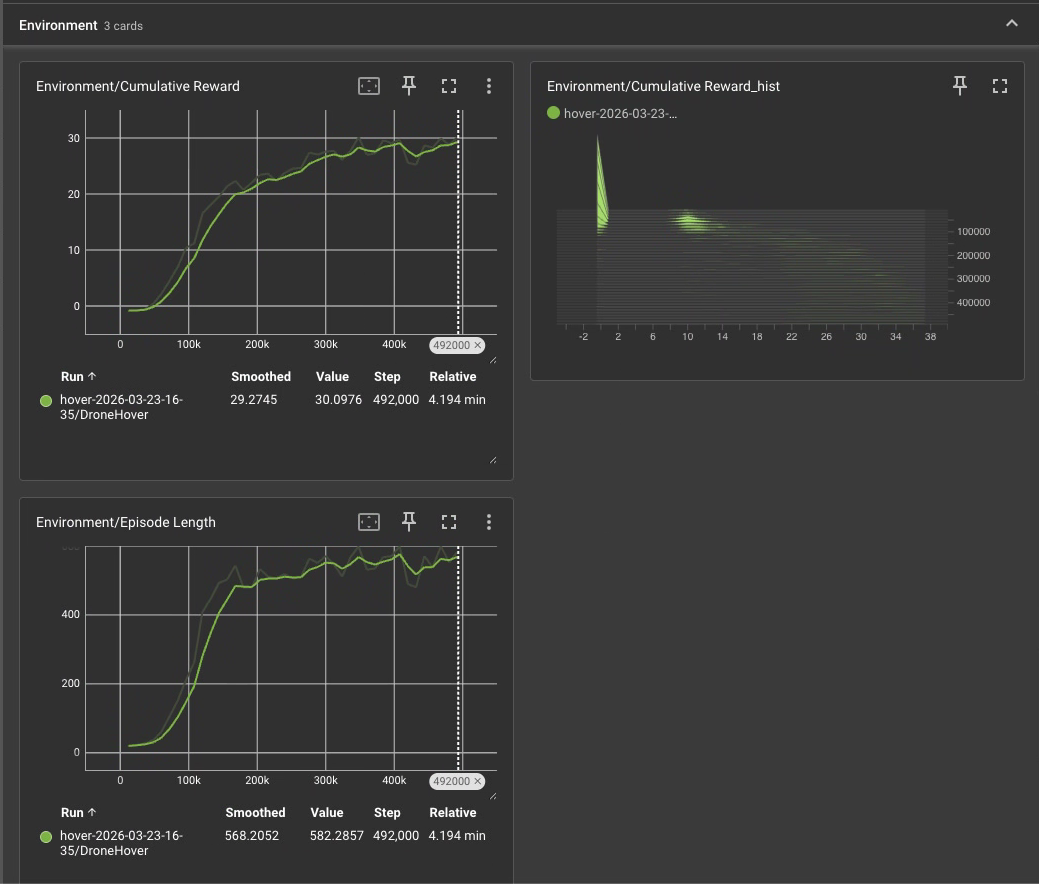
\includegraphics[width=1\linewidth]{img/result.png}
\end{figure}

Moreover, the use of a decision interval (DecisionRequester) enabled the control output to be updated at a lower frequency, resulting in smoother control signals compared to the PID-based approach, which aligns more closely with human perceptual capabilities (see Figure~\ref{fig:rl_hover}).

\begin{figure}[H]
    \caption{User interface prototype of the reinforcement learning agent.}\label{fig:rl_hover}
    \centering
    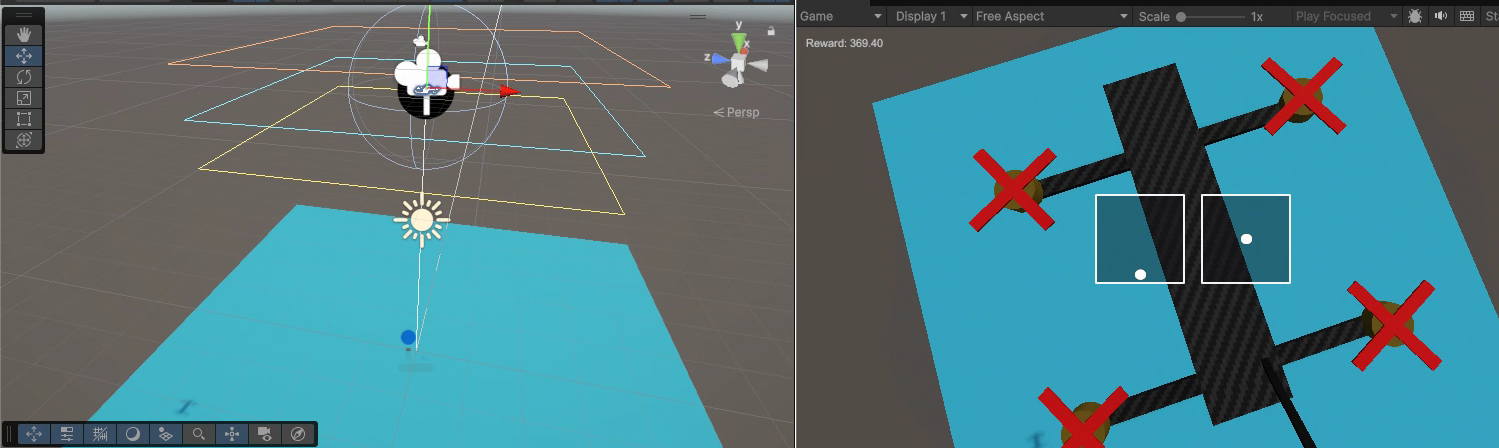
\includegraphics[width=1\linewidth]{img/hover.png}
\end{figure}

\paragraph{Analysis}

Although the RL agent achieved stable hovering in a simplified setting, several limitations were identified.

First, the approach did not scale well to more complex tasks such as path following. These tasks require a larger set of state variables (e.g., position, velocity, and angular motion in multiple axes), which increases the difficulty of training.

Second, the RL model behaved as a black-box system. Fine-tuning the behavior required extensive experimentation, and the relationship between parameters and performance was difficult to interpret.

Third, compared to the PID-based method, the RL approach required significantly more training time and computational resources, while not providing a clear advantage in control stability in the current study.

The RL-based approach is considered promising for future work. However, it requires a more systematic pipeline, such as data collection and state variable reduction (e.g., using principal component analysis), which is beyond the scope of the current study.